%% In the documentclass line, replace "noanswers" with "answers" to view the key.

\documentclass[noanswers]{exam}
\usepackage[utf8]{inputenc}

\title{Practice Problems}
\author{Chapter 3}
\date{STAT 3090}

\usepackage[bottom=2.2cm, left=2.2cm, right=2.2cm, top=2.2cm]{geometry}
%\usepackage[paperheight=11in, paperwidth=17in, margin=1in]{geometry}
\usepackage{dsfont}
\usepackage{amsmath}
\usepackage{amssymb}
\usepackage{amsthm}
\usepackage{array}
\usepackage{stmaryrd}
\usepackage{pgfplots}
\pgfplotsset{width=10cm,compat=1.9}
\usepackage{multicol}
\setlength{\columnsep}{1in}
\usepackage{nicefrac}

\usepackage{multirow}
\usepackage{enumitem}[shortlabels]
\usepackage{tabu}
\definecolor{purp}{RGB}{102,0,204}
\usepackage{tabularx}
\newcolumntype{C}{>{\centering\arraybackslash $}X<{$}}
\usepackage{wrapfig}
\usepackage[export]{adjustbox}


\makeatletter
\pagestyle{headandfoot}
\firstpageheader{\@date}{\@title}{\@author}
\firstpageheadrule
\runningfootrule
\runningfooter{}{\thepage\ / \numpages}{\@title}
\makeatother

\newcommand{\abs}[1]{\left|#1\right|}
\newcommand{\mat}[4]{\left( \begin{tabular}{>{$}c<{$} >{$}c<{$}} #1&#2 \\ #3&#4 \end{tabular} \right)}
\newcommand{\msc}[1]{\mathds{#1}}
\newcommand{\Z}{\mathds{Z}}
\newcommand{\R}{\mathds{R}}
\newcommand{\N}{\mathds{N}}
\newcommand{\Q}{\mathds{Q}}
\newcommand{\C}{\mathds{C}}
\newcommand{\so}{\implies}
\newcommand{\set}[2]{\left\{ #1 \:|\: #2 \right\}}
\newcommand{\bso}{\Longleftarrow}
\newcommand{\ra}{\rightarrow}
\newcommand{\gen}[1]{\left\langle #1 \right\rangle}
\newcommand{\olin}[1]{\overline{#1}}
\newcommand{\Img}[1]{\text{Im}\left(#1\right)}
\newcommand{\llra}{\longleftrightarrow}
\newcommand{\lra}{\longrightarrow}
\newcommand{\xra}[1]{\xrightarrow{#1}}
\newcommand{\wo}{\setminus}
\newcommand{\mcal}[1]{\mathcal{#1}}
\newcommand{\Aut}[1]{\text{Aut}\left(#1\right)}
\newcommand{\Inn}[1]{\text{Inn}\left(#1\right)}
\newcommand{\syl}[2]{\text{Syl}_{#1}(#2)}
\newcommand{\norm}[1]{\left\|#1\right\|}
\newcommand{\infnorm}[1]{\left\|#1\right\|_{\infty}}
\newcommand{\xn}{\{x_n\}}
\newcommand{\sig}{\sigma}
\newcommand{\id}{\text{id}}
\newcommand{\ep}{\epsilon}
\newcommand{\st}{\text{ s.t. }}
\newcommand{\ran}[1]{\text{Ran}(#1)}
\newcommand{\nCr}[2]{\binom{#1}{#2}}
\newcommand{\Exr}[1]{\paragraph{Exercise #1:}}
\newcommand{\pg}{\paragraph{}}
\newcommand{\ulin}[1]{\underline{#1}}
\newcommand{\tc}[1]{\textcolor{purp}{#1}}

% Solution Specs
\unframedsolutions
\renewcommand{\solutiontitle}{}
\SolutionEmphasis{\color{purp}}
\CorrectChoiceEmphasis{\color{purp}\bfseries}
\renewcommand{\arraystretch}{2}
\setlength\fillinlinelength{0in}

%\begin{solution}[\stretch{1}]
%	hurp durp flurp
%\end{solution}

%\pagestyle{empty}

\begin{document}

%\noindent\begin{tabular}{@{}p{.3in}p{3in}@{}}
%Name: & \hrulefill
%\end{tabular}
%
%\noindent\begin{tabular}{@{}p{1.05in}p{3.2in}@{}}
%Group Members: & \hrulefill
%\end{tabular}

\begin{questions} 
	
	\question Consider the following scores that Miss Frizzle's students made on their Biology final exam.
	
	\begin{center}
    \begin{tabular}{c c c c c c c c c c c c c c c c}
        51 & 57 & 59 & 62 & 64 & 65 & 65 & 68 & 71 & 72 & 74 & 78 & 78 & 78 & 79 & 80\\   
        83 & 83 & 85 & 86 & 87 & 87 & 87 & 89 & 89 & 90 & 91 & 93 & 93 & 94 & 95 & 97\\  
        97 & 98 & 98 & 99 & 100\\
    \end{tabular}
\end{center}
	
	\begin{parts}
	
	\part You determine that these quantitative data would best be organized in bins with a width of ten to correspond to letter grades. Complete the following table with the appropriate \textbf{frequencies}, \textbf{relative frequencies}, and \textbf{cumulative relative frequencies}.
	
	\begin{center}
\begin{tabular}{|*{4}{c|}}
\hline
\textbf{Student Scores} & \textbf{Frequency} & \textbf{Relative Frequency} & \textbf{Cumulative Relative Frequency}\\
\hline
[50,60) & \fillin[$3$] & \fillin[$\frac{3}{37} = 0.0811$] & \fillin[$\frac{3}{37} = 0.0811$] \\
\hline
[60,70) & \fillin[$5$] & \fillin[$\frac{5}{37} = 0.1351$] & \fillin[$\frac{8}{37} = 0.2162$] \\
\hline
[70,80) & \fillin[$7$] & \fillin[$\frac{7}{37} = 0.1892$] & \fillin[$\frac{15}{37} = 0.4054$] \\
\hline
[80,90) & \fillin[$10$] & \fillin[$\frac{10}{37} = 0.2703$] & \fillin[$\frac{25}{37} = 0.6757$] \\
\hline
[90,100] & \fillin[$12$] & \fillin[$\frac{12}{37} = 0.3243$] & \fillin[$\frac{37}{37} = 1.0000$] \\
\hline
\end{tabular}
\end{center}
	
	\vspace{3mm}	
	
	\part What proportion of students scored \textbf{less than a C} on the exam?
	
	\begin{solution}[\stretch{1}]
	
			\vspace{3mm}		
			$\displaystyle \frac{8}{37}=0.2162$ (or 21.62\%) of students scored below a C (below 70).

			\vspace{3mm}		
			
		\end{solution}
	
	\vspace{3mm}	
	
	\part A 60\% or higher is required on the final exam to pass the course. What proportion of students are \textbf{eligible to pass}?
	
	\begin{solution}[\stretch{1}]
	
			\vspace{3mm}		
			$1-\frac{3}{37}=\frac{34}{37}=0.9189$ (or 91.89\%) of students are eligible to pass the course.

			\vspace{3mm}		
			
		\end{solution}	
		
		\vspace{3mm}
		
		
		
	\part Sketch a \textbf{stem and leaf plot} of the data. Include a title and key.
	
	\begin{solution}[\stretch{3}]
	
			\vspace{3mm}		
			Key: 5 $|$ 1 $=$ exam score of 51
			
			\vspace{1mm}
			
			\begin{tabular}{r|l}
			5 & 1 7 9 \\
			6 & 2 4 5 5 8\\ 
			7 & 1 2 4 8 8 8 9\\
			8 & 0 3 3 5 6 7 7 7 9 9\\
			9 & 0 1 3 3 4 5 7 7 8 8 9\\
			10 & 0			
			\end{tabular}

			\vspace{3mm}		
			
		\end{solution}
	
	\end{parts}
	
	
	
	\newpage
	

\question Dwight is interested in determining whether a preservative is effective in reducing discoloration in frozen
beets from Schrute Farms. A sample of 50 ripe beets was chosen from the most recent crop, and each beet was prepared for freezing and placed in a Ziploc bag. The preservative was added to the beets in 25 randomly assigned bags, then all the bags were sealed and stored at 0 $^\circ$C for a period of 4 months. At the end of this time, after the beets were thawed, Dwight's cousin Mose rated each beet's discoloration from
1 to 10, with a low score indicating little discoloration. The dot plots below show the distributions of the discoloration rating for the control and treatment groups.
	
	\begin{center}
		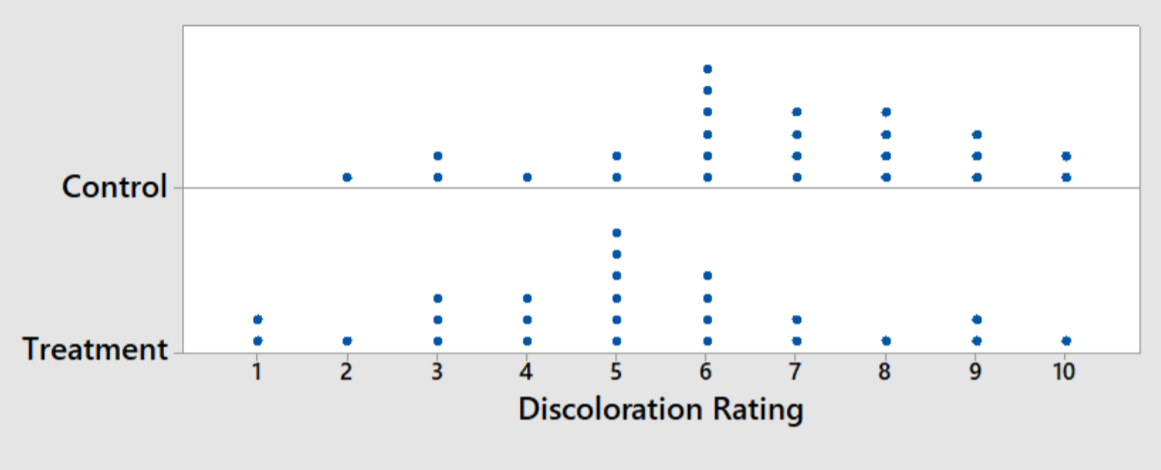
\includegraphics[scale=.4]{STAT_3090_Ch3_dotplot.PNG}
	\end{center}
	
	\vspace{3mm}
	
	\begin{parts}
		\part Identify the \textbf{explanatory variable}.
		
		\begin{solution}[\stretch{3}]
	
			\vspace{3mm}		
			Whether or not preservative was used (yes/no)

			\vspace{3mm}		
			
		\end{solution}
		
		\part Identify the \textbf{response variable}.
		
		\begin{solution}[\stretch{3}]
	
			\vspace{3mm}		
			Amount of discoloration (1--10)

			\vspace{3mm}		
			
		\end{solution}
		
		\part How many beet bags received a rating of \textbf{3 or less} in the control group? In the treatment group?
		
		\begin{solution}[\stretch{3}]
	
			\vspace{3mm}		
			Three bags received a rating of 3 or less in the control group, while six bags received a 3 or less in the treatment group.

			\vspace{3mm}		
			
		\end{solution}
		
		\part How many beet bags received a rating of \textbf{7 or more} in the control group? In the treatment group?
		
		\begin{solution}[\stretch{3}]
	
			\vspace{3mm}		
			Thirteen bags received a rating of 7 or more in the control group, while six received a 7 or more in the treatment group.

			\vspace{3mm}		
			
		\end{solution}
		
\part Graphical summaries of data can give us a ``picture'' of the general trends within the data. Based on what you can see in the dot plots for Dwight's beet experiment, do you think the preservative was effective? \textbf{Justify} your answer.
		
		\begin{solution}[\stretch{5}]
	
			\vspace{3mm}		
			In general, we see more observations with \underline{low} discoloration ratings and fewer observations with \underline{high} discoloration ratings in the treatment group compared to the control group, which would suggest that the preservative treatment might be effective. (Good news for Schrute Farms!) 

			\vspace{3mm}		
			
		\end{solution}		
		
	\end{parts}

\end{questions}

%-----------------------------------------------------------------------------%

\end{document}
